\documentclass[a4paper,11pt]{book}
%\documentclass[a4paper,11pt,makeidx]{book} <== may need this to generate index

%  makeindex NEMO_book  <== to regenerate the index
%  bibtex    NEMO_book	<== to generate  the bibliography

%\usepackage[french]{babel}
%\usepackage{color}
\usepackage{rotating, graphicx}			           % allows insertion of pictures
%\usepackage{graphics}			                   % allows insertion of pictures
\graphicspath{{Figures/}}                                  % Set global directory for pictures
\DeclareGraphicsExtensions{.pdf,.eps}                      % Use .eps for LaTeX2HTML
%\usepackage{xcolor}                                       % Incompatibility with color -> graphicx
\usepackage[capbesideposition={top,center}]{floatrow}      % allows captions
\floatsetup[table]{style=plaintop}                         % beside pictures
\usepackage[margin=10pt,font={small},                      % Gives small font for captions
labelsep=colon,labelfont={bf}]{caption}                    %
\usepackage{enumitem}                                      % allows non-bold description items
\usepackage{longtable}                                     % allows multipage tables
%\usepackage{colortbl}                                     % gives coloured panels behind table columns

%hyperref
\usepackage[pdftitle={NEMO ocean engine},pdfauthor={Gurvan Madec},pdfstartview=FitH,
bookmarks=true,bookmarksopen=true,breaklinks=true,colorlinks=true,
linkcolor=blue,anchorcolor=blue,citecolor=blue,filecolor=blue,menucolor=blue,urlcolor=blue]{hyperref}
% pdfsubject={The preprint document class
%   elsart},% pdfkeywords={diapycnal diffusion,numerical mixing,z-level models},%%  usage of exteranl hyperlink :  \href{mailto:my_address@wikibooks.org}{my\_address@wikibooks.org}
%                                                 \url{http://www.wikibooks.org}
%                                     or         \href{http://www.wikibooks.org}{wikibooks home}


%%%% page styles etc................
\usepackage{fancyhdr}
\pagestyle{fancy}
% with this we ensure that the chapter and section
% headings are in lowercase.
\renewcommand{\chaptermark}[1]{\markboth{#1}{}}
\renewcommand{\sectionmark}[1]{\markright{\thesection.\ #1}}
\fancyhf{}             % delete current setting for header and footer
\fancyhead[LE,RO]{\bfseries\thepage}
\fancyhead[LO]{\bfseries\hspace{-0em}\rightmark}
\fancyhead[RE]{\bfseries\leftmark}
\renewcommand{\headrulewidth}{0.5pt}
\renewcommand{\footrulewidth}{0pt  }
\addtolength{\headheight}{2.6pt}   % make space for the rule
%\addtolength{\headheight}{1.6pt}   % make space for the rule
% get rid of headers on plain pages
\fancypagestyle{plain}{\fancyhead{}\renewcommand{\headrulewidth}{0pt}}


%%%%  Section number in Margin.......
% typeset the number of each section in the left margin, with the start of each instance of
% sectional heading text aligned with the left hand edge of  the body text.
\makeatletter
\def\@seccntformat#1{\protect\makebox[0pt][r]{\csname the#1\endcsname\quad}}
\makeatother

% Leave blank pages completely empty, w/o header
\makeatletter
\def\cleardoublepage{\clearpage\if@twoside \ifodd\c@page\else
  \hbox{}
  \vspace*{\fill}
  \vspace{\fill}
  \thispagestyle{empty}
  \newpage
  \if@twocolumn\hbox{}\newpage\fi\fi\fi}
\makeatother

%%%% define the chapter  style ................
\usepackage{minitoc}				%In French : \usepackage[french]{minitoc}
%\usepackage{mtcoff}				% invalidate the use of minitocs
\usepackage{fancybox}

\makeatletter
\def\LigneVerticale{\vrule height 5cm depth 2cm\hspace{0.1cm}\relax}
\def\LignesVerticales{%
  \let\LV\LigneVerticale\LV\LV\LV\LV\LV\LV\LV\LV\LV\LV}
\def\GrosCarreAvecUnChiffre#1{%
  \rlap{\vrule height 0.8cm width 1cm depth 0.2cm}%
 \rlap{\hbox to 1cm{\hss\mbox{\color{white} #1}\hss}}%
  \vrule height 0pt width 1cm depth 0pt}
\def\GrosCarreAvecTroisChiffre#1{%
  \rlap{\vrule height 0.8cm width 1.6cm depth 0.2cm}%
 \rlap{\hbox to 1.5cm{\hss\mbox{\color{white} #1}\hss}}%
  \vrule height 0pt width 1cm depth 0pt}

\def\@makechapterhead#1{\hbox{%
   \huge
    \LignesVerticales
    \hspace{-0.5cm}%
    \GrosCarreAvecUnChiffre{\thechapter}
    \hspace{0.2cm}\hbox{#1}%
%    \GrosCarreAvecTroisChiffre{\thechapter}
%    \hspace{1cm}\hbox{#1}%
%}\par\vskip 2cm}
}\par\vskip 1cm}
\def\@makeschapterhead#1{\hbox{%
   \huge
    \LignesVerticales
    %\hspace{0.5cm}%
    \hbox{#1}%
}\par\vskip 2cm}
\makeatother

%\def\thechapter{\Roman{chapter}}   	% chapter number to be Roman


%%%%           Mathematics...............
%\documentclass{amsart}
\usepackage{xspace}                              % helpd ensure correct spacing after macros
\usepackage{latexsym,amssymb,amsmath}
\allowdisplaybreaks[1]				% allow page breaks in the middle of equations
\usepackage{TexFiles/Styles/math_abbrev}    % use maths shortcuts

\usepackage{times}			 	 % use times font for text
%\usepackage{mathtime}                          % font for illustrator to work (belleek fonts )
%\usepackage[latin1]{inputenc}                % allows some unicode removed (agn)


%%% essai commande
\newcommand{\nl}[1]{\texttt{\small{\textcolor{blue}{#1}}}}
\newcommand{\nlv}[1]{\texttt{\footnotesize#1}\xspace}
\newcommand{\smnlv}[1]{\texttt{\scriptsize#1}\xspace}

%%%% namelist & code display................................
\usepackage{alltt,verbatim}  	%%  alltt & verbatim for namelist
% namelists
\newcommand{\namdisplay}[1]{\begin{alltt}{\tiny\verbatiminput{Namelists/#1}}\end{alltt}\vspace{-10pt}}
\newcommand{\namtools}[1]{\begin{alltt}{\tiny\verbatiminput{Namelists/#1}}\end{alltt}\vspace{-10pt}}
% code display
%\newcommand{\codedisplay} [1] {\begin{alltt}{\tiny {\begin{verbatim} {#1}} \end{verbatim}} \end{alltt}      }



%%%% commands for working with text................................
% command to "comment out" portions of text ({} argument) or not ({#1} argument)
\newcommand{\amtcomment}[1]{}   	% command to "commented out" portions of text or not (#1 in argument)
\newcommand{\sgacomment}[1]{}   	% command to "commented out" portions of
\newcommand{\gmcomment}[1]{}   	% command to "commented out" portions of
%                                    				% text that span line breaks
%Red (NR) or Yellow(WARN)
%\newcommand{\NR}   {\colorbox{red}   {#1}}
%\newcommand{\WARN} {\colorbox{yellow}{#1}}



%%% index commands......................
\usepackage{makeidx}
%\usepackage{showidx}				% show the index entry

\newcommand{\mdl}[1]{\textit{#1.F90}\index{Modules!#1}}	%module (mdl)
\newcommand{\rou}[1]{\textit{#1}\index{Routines!#1}}	%module (routine)
\newcommand{\hf}[1]{\textit{#1.h90}\index{h90 file!#1}}	%module (h90 files)
\newcommand{\ngn}[1]{\textit{#1}\index{Namelist Group Name!#1}}	%namelist name (nampar)
\newcommand{\np}[1]{\textit{#1}\index{Namelist variables!#1}}        %namelist variable
\newcommand{\jp}[1]{\textit{#1}\index{Model parameters!#1}}	%model parameter (jp)
\newcommand{\pp}[1]{\textit{#1}\index{Model parameters!#1}} 	%namelist parameter (pp)
\newcommand{\ifile}[1]{\textit{#1.nc  }\index{Input NetCDF files!#1.nc}}	%input NetCDF files (.nc)
\newcommand{\key}[1]{\textbf{key\_#1}\index{CPP keys!key\_#1}}	%key_cpp (key)
\newcommand{\NEMO}{\textit{NEMO}\xspace}	%NEMO (nemo)

%%%%   Bibliography   .............
\usepackage[nottoc,notlof,notlot]{tocbibind}
\usepackage[square,comma]{natbib}
\bibpunct{[}{]}{,}{a}{}{;}                           %suppress "," after "et al."
\providecommand{\bibfont}{\small}

\usepackage{subfiles}                          % Separate compilation of chapters from whole manual
%\newcommand{\onlyinsubfile}[1]{#1}             % New commands for printing parts according to
%\newcommand{\notinsubfile}[1]{}                % the file being compiled
% Commands to use in the documentfile
%\renewcommand{\onlyinsubfile}[1]{}                      % Appears only if chapter   .tex file is compiled
%\renewcommand{\notinsubfile}[1]{#1}                     %    "    ""   "" NEMO_book .tex file is compiled

\DeclareMathAlphabet{\mathpzc}{OT1}{pzc}{m}{it}


\begin{document}

\title{Draft description of NEMO wetting and drying scheme:     29 November 2017 }

\author{ Enda O'Dea, Hedong Liu, Jason Holt, Andrew Coward  and Michael J. Bell  }

%------------------------------------------------------------------------
% End of temporary latex header (to be removed) 
%------------------------------------------------------------------------

% ================================================================
% Chapter Ocean Dynamics (DYN)
% ================================================================
\chapter{Ocean Dynamics (DYN)}
\label{DYN}
\minitoc

% add a figure for  dynvor ens, ene latices

$\ $\newline    % force a new ligne

% ================================================================
% Wetting and drying 
% ================================================================
 
%----------------------------------------------------------------------------------------
%      The WAD test cases
%----------------------------------------------------------------------------------------
\section   [The WAD test cases (\textit{usrdef\_zgr})]
			{The WAD test cases (\mdl{usrdef\_zgr})}
\label{WAD_test_cases}

This section contains details of the seven test cases that can be run as part of the
WAD\_TEST\_CASES configuration. All the test cases are shallow (less than 10m deep),
basins or channels with 4m high walls and some of topography that can wet and dry up to
2.5m above sea-level. The horizontal grid is uniform with a 1km resolution and measures
52km by 34km. These dimensions are determined by a combination of code in the
\mdl{usrdef\_nam} module located in the WAD\_TEST\_CASES/MY\_SRC directory and setting
read in from the namusr\_def namelist. The first six test cases are closed systems with no
rotation or external forcing and motion is simply initiated by an initial ssh slope. The
seventh test case introduces and open boundary at the right-hand end of the channel which
is forced with sinousoidally varying ssh and barotropic velocities.

\namdisplay{nam_wad_usr}

The $\mathrm{nn\_wad\_test}$ parameter can takes values 1 to 7 and it is this parameter
that determines which of the test cases will be run. Most cases can be run with the
default settings but the simple linear slope cases (tests 1 and 5) can be run with lower
values of $\mathrm{rn\_wdmin1}$. Any recommended changes to the default namelist settings
will be stated in the individual subsections.

Test case 7 requires additional {\tt namelist\_cfg} changes to activate the open boundary
and lengthen the duration of the run (in order to demonstrate the full forcing cycle).
There is also a simple python script which needs to be run in order to generate the
boundary forcing files.  Full details are given in subsection (\ref{WAD_test_case7}).

\clearpage
\subsection [WAD test case 1 : A simple linear slope]
                    {WAD test case 1 : A simple linear slope}
\label{WAD_test_case1}

The first test case is a simple linear slope (in the x-direction, uniform in y) with an
adverse SSH gradient that, when released, creates a surge up the slope. The parameters are
chosen such that the surge rises above sea-level before falling back and oscillating
towards an equilibrium position. This case can be run with $\mathrm{rn\_wdmin1}$ values as
low as 0.075m. I.e. the following change may be made to the default values in {\tt
namelist\_cfg} (for this test only):

\namdisplay{nam_wad_tc1}

%>>>>>>>>>>>>>>>>>>>>>>>>>>>>>>>>>>>>>>>>>>>>
\begin{figure}[htb] \begin{center}
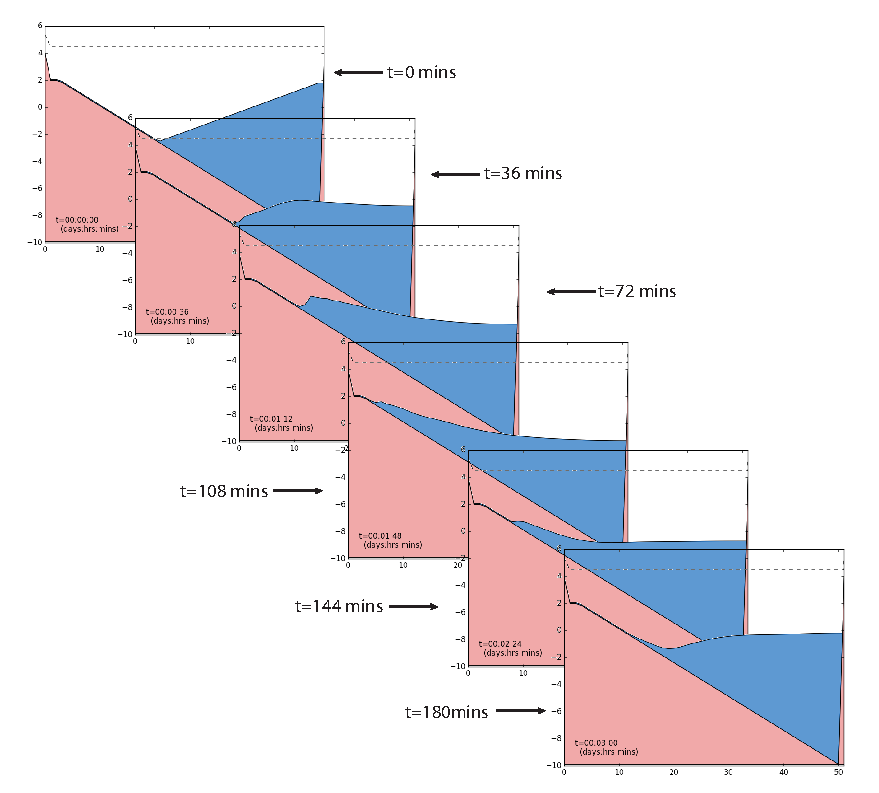
\includegraphics[width=0.8\textwidth]{Fig_WAD_TC1}
\caption{ \label{Fig_WAD_TC1}
The evolution of the sea surface height in WAD\_TEST\_CASE 1 from the initial state (t=0)
over the first three hours of simulation. Note that in this time-frame the resultant surge
reaches to nearly 2m above sea-level before retreating.}
\end{center}\end{figure}
%>>>>>>>>>>>>>>>>>>>>>>>>>>>>>>>>>>>>>>>>>>>>

\clearpage
\subsection [WAD test case 2 : A parabolic channel ]
                    {WAD test case 2 : A parabolic channel}
\label{WAD_test_case2}

The second and third test cases use a closed channel which is parabolic in x and uniform
in y.  Test case 2 uses a gentler initial SSH slope which nevertheless demonstrates the
ability to wet and dry on both sides of the channel. This solution requires values of
$\mathrm{rn\_wdmin1}$ at least 0.3m ({\it Q.: A function of the maximum topographic
slope?})

\namdisplay{nam_wad_tc2}

%>>>>>>>>>>>>>>>>>>>>>>>>>>>>>>>>>>>>>>>>>>>>
\begin{figure}[htb] \begin{center}
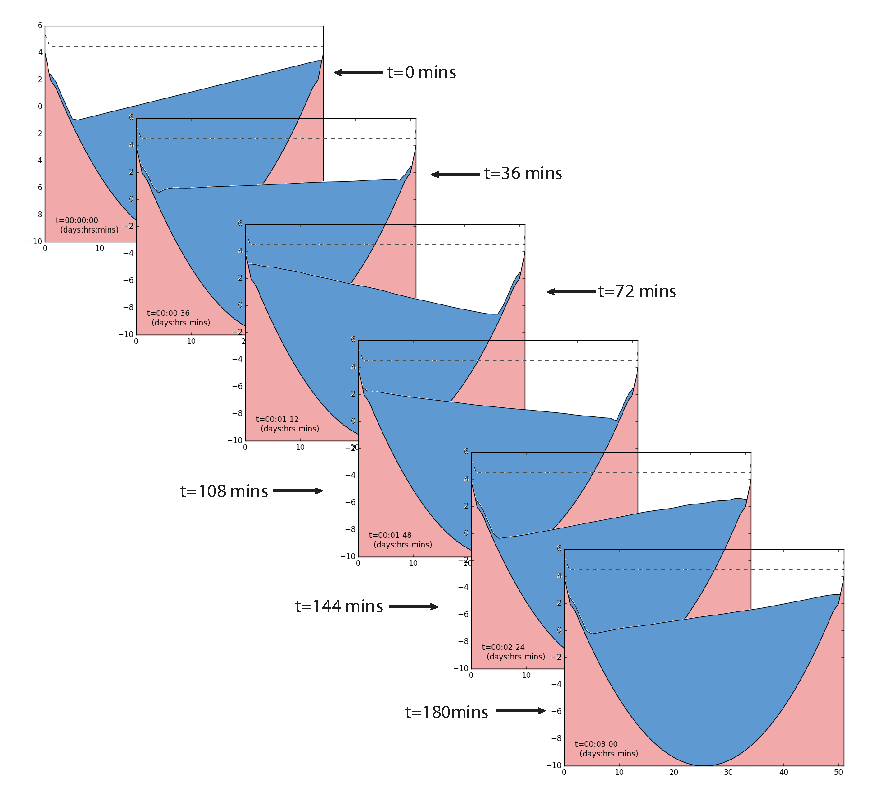
\includegraphics[width=0.8\textwidth]{Fig_WAD_TC2}
\caption{ \label{Fig_WAD_TC2}
The evolution of the sea surface height in WAD\_TEST\_CASE 2 from the initial state (t=0)
over the first three hours of simulation. Note that in this time-frame the resultant sloshing
causes wetting and drying on both sides of the parabolic channel.}
\end{center}\end{figure}
%>>>>>>>>>>>>>>>>>>>>>>>>>>>>>>>>>>>>>>>>>>>>

\clearpage
\subsection [WAD test case 3 : A parabolic channel (extreme slope) ]
                    {WAD test case 3 : A parabolic channel (extreme slope)}
\label{WAD_test_case3}

Similar to test case 2 but with a steeper initial SSH slope. The solution is similar but more vigorous.

\namdisplay{nam_wad_tc3}

%>>>>>>>>>>>>>>>>>>>>>>>>>>>>>>>>>>>>>>>>>>>>
\begin{figure}[htb] \begin{center}
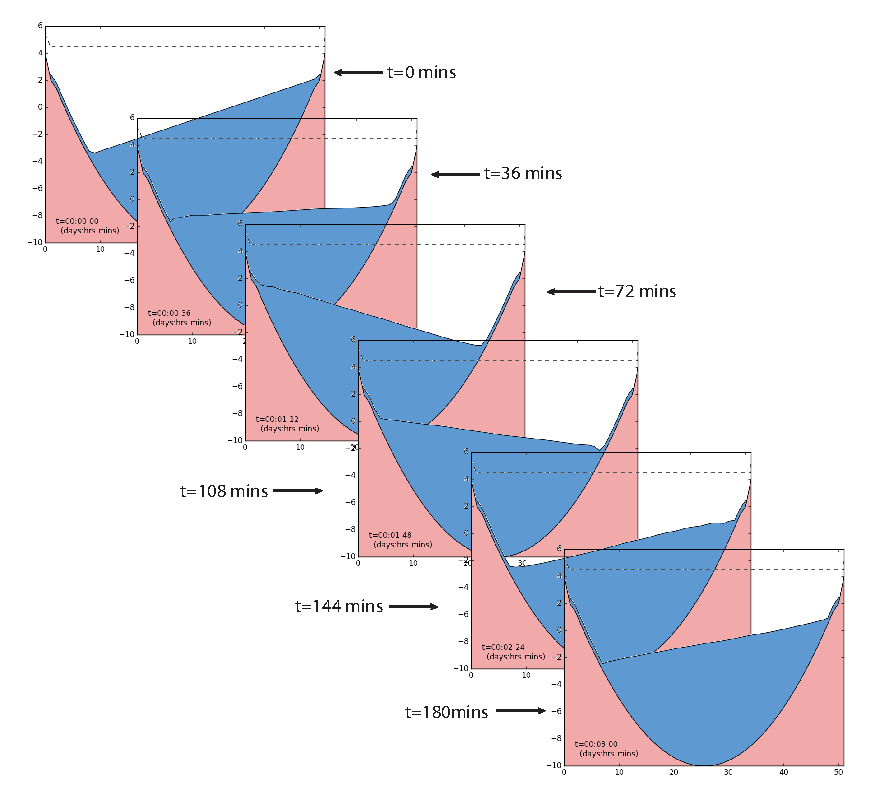
\includegraphics[width=0.8\textwidth]{Fig_WAD_TC3}
\caption{ \label{Fig_WAD_TC3}
The evolution of the sea surface height in WAD\_TEST\_CASE 3 from the initial state (t=0)
over the first three hours of simulation. Note that in this time-frame the resultant sloshing
causes wetting and drying on both sides of the parabolic channel.}
\end{center}\end{figure}
%>>>>>>>>>>>>>>>>>>>>>>>>>>>>>>>>>>>>>>>>>>>>

\clearpage
\subsection [WAD test case 4 : A parabolic bowl ]
                    {WAD test case 4 : A parabolic bowl}
\label{WAD_test_case4}

Test case 4 includes variation in the y-direction in the form of a parabolic bowl. The
initial condition is now a raised bulge centred over the bowl. Figure \ref{Fig_WAD_TC4}
shows a cross-section of the SSH in the X-direction but features can be seen to propagate
in all directions and interfere when return paths cross.

\namdisplay{nam_wad_tc4}

%>>>>>>>>>>>>>>>>>>>>>>>>>>>>>>>>>>>>>>>>>>>>
\begin{figure}[htb] \begin{center}
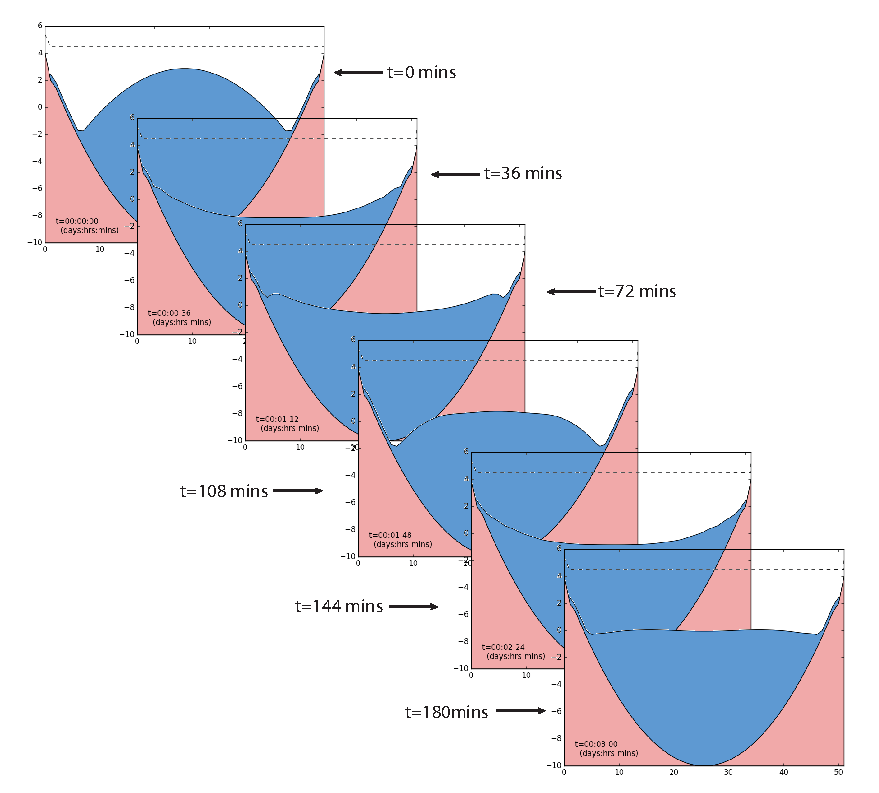
\includegraphics[width=0.8\textwidth]{Fig_WAD_TC4}
\caption{ \label{Fig_WAD_TC4}
The evolution of the sea surface height in WAD\_TEST\_CASE 4 from the initial state (t=0)
over the first three hours of simulation. Note that this test case is a parabolic bowl with
variations occurring in the y-direction too (not shown here).}
\end{center}\end{figure}
%>>>>>>>>>>>>>>>>>>>>>>>>>>>>>>>>>>>>>>>>>>>>

\clearpage
\subsection [WAD test case 5 : A double slope with shelf channel ]
                    {WAD test case 5 : A double slope with shelf channel}
\label{WAD_test_case5}

Similar in nature to test case 1 but with a change in slope and a mid-depth shelf.

\namdisplay{nam_wad_tc5}

%>>>>>>>>>>>>>>>>>>>>>>>>>>>>>>>>>>>>>>>>>>>>
\begin{figure}[htb] \begin{center}
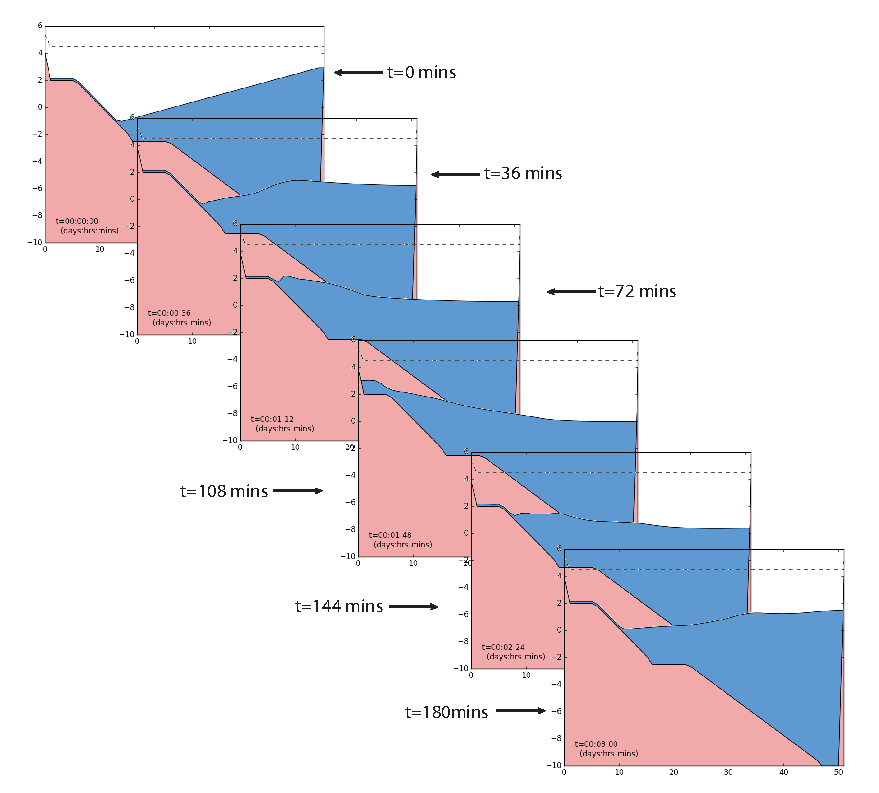
\includegraphics[width=0.8\textwidth]{Fig_WAD_TC5}
\caption{ \label{Fig_WAD_TC5}
The evolution of the sea surface height in WAD\_TEST\_CASE 5 from the initial state (t=0)
over the first three hours of simulation. The surge resulting in this case wets to the full 
depth permitted (2.5m above sea-level) and is only halted by the 4m high side walls.}
\end{center}\end{figure}
%>>>>>>>>>>>>>>>>>>>>>>>>>>>>>>>>>>>>>>>>>>>>

\clearpage
\subsection [WAD test case 6 : A parabolic channel with central bar ]
                    {WAD test case 6 : A parabolic channel with central bar}
\label{WAD_test_case6}

Test cases 1 to 5 have all used uniform T and S conditions. The dashed line in each plot
shows the surface salinity along the y=17 line which remains satisfactorily constant. Test
case 6 introduces variation in salinity by taking a parabolic channel divided by a central
bar (gaussian) and using two different salinity values in each half of the channel. This
step change in salinity is initially enforced by the central bar but the bar is
subsequently over-topped after the initial SSH gradient is released. The time series in
this case shows the SSH evolution with the water coloured according to local salinity
values. Encroachment of the high salinity (red) waters into the low salinity (blue) basin
can clearly be seen.

\namdisplay{nam_wad_tc6}

%>>>>>>>>>>>>>>>>>>>>>>>>>>>>>>>>>>>>>>>>>>>>
\begin{figure}[htb] \begin{center}
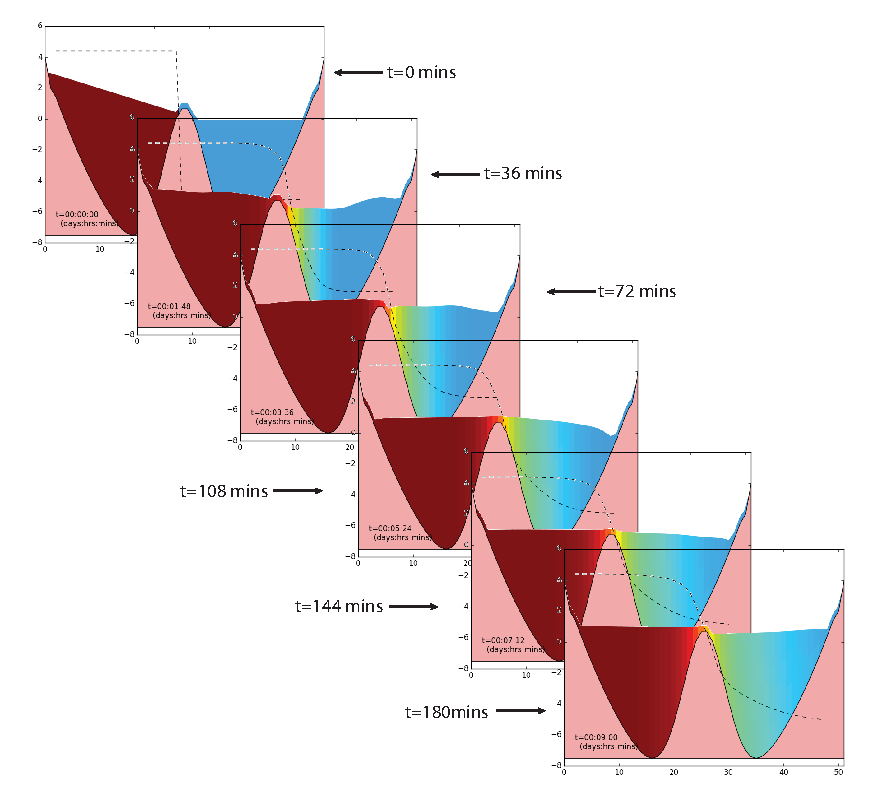
\includegraphics[width=0.8\textwidth]{Fig_WAD_TC6}
\caption{ \label{Fig_WAD_TC6}
The evolution of the sea surface height in WAD\_TEST\_CASE 6 from the initial state (t=0)
over the first three hours of simulation. Water is coloured according to local salinity
values. Encroachment of the high salinity (red) waters into the low salinity (blue) basin
can clearly be seen although the largest influx occurs early in the sequence between the
frames shown.}
\end{center}\end{figure}
%>>>>>>>>>>>>>>>>>>>>>>>>>>>>>>>>>>>>>>>>>>>>

\clearpage
\subsection [WAD test case 7 : A double slope with shelf, open-ended channel ]
                    {WAD test case 7 : A double slope with shelf, open-ended channel}
\label{WAD_test_case7}

Similar in nature to test case 5 but with an open boundary forced with a sinusoidally
varying ssh. This test case has been introduced to emulate a typical coastal application
with a tidally forced open boundary. The bathymetry and setup is identical to test case 5
except the right hand end of the channel is now open and has simple ssh and barotropic
velocity boundary conditions applied at the open boundary. Several additional steps and
namelist changes are required to run this test.

\namdisplay{nam_wad_tc7}

In addition, the boundary condition files must be generated using the python script
provided.

\begin{verbatim}
python ./makebdy_tc7.py
\end{verbatim}

will create the following boundary files for this test (assuming a suitably configured
python environment: python2.7 with netCDF4 and numpy):

\begin{verbatim}
  bdyssh_tc7_m12d30.nc   bdyuv_tc7_m12d30.nc
  bdyssh_tc7_m01d01.nc   bdyuv_tc7_m01d01.nc
  bdyssh_tc7_m01d02.nc   bdyuv_tc7_m01d02.nc
  bdyssh_tc7_m01d03.nc   bdyuv_tc7_m01d03.nc
\end{verbatim}

These are sufficient for up to a three day simulation; the script is easily adapted if
longer periods are required.

%>>>>>>>>>>>>>>>>>>>>>>>>>>>>>>>>>>>>>>>>>>>>
\begin{sidewaysfigure}[htb] \begin{center}
\includegraphics[width=0.8\textwidth]{Fig_WAD_TC7}
\caption{ \label{Fig_WAD_TC7}
The evolution of the sea surface height in WAD\_TEST\_CASE 7 from the initial state (t=0)
over the first 24 hours of simulation. After the initial surge the solution settles into a
simulated tidal cycle with an amplitude of 5m. This is enough to repeatedly wet and dry
both shelves.}

\end{center}\end{sidewaysfigure}
%>>>>>>>>>>>>>>>>>>>>>>>>>>>>>>>>>>>>>>>>>>>>


% ================================================================

%\bibliographystyle{wileyqj}
%\bibliographystyle{../../../doc/latex/NEMO/main/ametsoc.bst}
%\bibliography{references}

\end{document}
